\documentclass[a4paper,12pt]{article}
%\documentclass[a4paper,fontsize=13pt]{scrartcl}

\usepackage{tabularx}
\usepackage{amsmath}
\usepackage[utf8]{inputenc}
\usepackage{multicol}
\usepackage{amsmath, amssymb, amsthm}
\usepackage{graphicx}
\usepackage{enumitem}
\usepackage{array}
\usepackage[left=2cm, right=2cm, top=2cm, bottom=2cm]{geometry}
\usepackage{fancyhdr}
\usepackage{xfp}
\usepackage{pgf}
\usepackage{tikz}

\usepackage{graphicx}
\usepackage{fancyhdr}
\setlength{\headheight}{28pt} % genug Platz für das Logo
\pagestyle{fancy}
\fancyhf{} % alles leeren
\fancyhead[L]{\includegraphics[height=1.2cm]{logo.png}}
\fancyhead[C]{\small Potenzfunktionen \ (Kl. G10B)}
\fancyhead[R]{\small Name:\ \rule{2.8cm}{0.4pt}}
\fancyfoot[C]{\thepage}

\fancyfoot[C]{Seite \thepage \enspace\textbullet\enspace J.\,Mycan \textcopyright~15.Dez.2025 *Klassenarbeit 45 min.*}

\renewcommand{\footrulewidth}{0.4pt}




%\pagestyle{fancy}
%\lhead{Klassenarbeit 45min.}
%\chead{Heinrich-von-Kleist-Schule}
%\rhead{Mathematik - G8A}
%\lfoot{}
%\cfoot{Seite \thepage}
%\rfoot{}

\newcommand{\punkteA}{12}
\newcommand{\punkteB}{8}
\newcommand{\punkteC}{9}
\newcommand{\punkteD}{15}
\newcommand{\punkteE}{8}
%\newcommand{\punkteF}{12}

\newcommand{\maxSumme}{52}
\newcommand{\noteEinsMin}{\fpeval{round(\maxSumme * 0.95,0)}}
\newcommand{\noteZweiMin}{\fpeval{round(\maxSumme * 0.80,0)}}
\newcommand{\noteDreiMin}{\fpeval{round(\maxSumme * 0.65,0)}}
\newcommand{\noteVierMin}{\fpeval{round(\maxSumme * 0.45,0)}}
\newcommand{\noteFunfMin}{\fpeval{round(\maxSumme * 0.20,0)}}
\newcommand{\noteSechsMin}{0}

\newcommand{\summe}{%
	\pgfmathparse{\punkteA + \punkteB + \punkteC + \punkteD + \punkteE}%
	\pgfmathprintnumber{\pgfmathresult}}

\begin{document}
	
%	\begin{center}
%		\textbf{Klassenarbeit - Lineare Funktionen und LGS}
%	\end{center}
	
%	\textbf{Vor- und Nachname:} \underline{\hspace{10cm}}\\[0.1cm]
Die Lösungen sowie Lösungswege sollen klar strukturiert und gut nachvollziehbar sein. Zeige alle Zwischenschritte und markiere das Endergebnis deutlich. Vereinfache Ergebnisse soweit möglich. \\
	
% -------------------------------------------------
% Aufgabe 1 (NEU)
% -------------------------------------------------
\textbf{Aufgabe 1 (12 Punkte)}\\
Bestimme jeweils eine Funktionsgleichung einer quadratischen Funktion in \emph{Scheitelpunktform}.
Nutze die Angaben sinnvoll und rechne nachvollziehbar.

\begin{enumerate}
	\item[a)] Die Parabel hat den Scheitelpunkt \(S(2\mid 1)\) und verläuft durch den Punkt \(P(0\mid 5)\).
	Stelle die Funktionsgleichung in Scheitelpunktform auf.
	
	\item[b)] Gegeben ist die Funktion in Produktform
	\[
	g(x) = -(x-1)(x+3).
	\]
	Bringe \(g(x)\) in die Scheitelpunktform.
	
	\item[c)] Eine Parabel besitzt die Nullstellen \(x_1=-1\) und \(x_2=5\) und schneidet die \(y\)-Achse bei \((0\mid -5)\).
	Bestimme die Funktionsgleichung in Scheitelpunktform.
\end{enumerate}


% -------------------------------------------------
% Aufgabe 2
% -------------------------------------------------
\textbf{Aufgabe 2 (10 Punkte)}\\
Ein Landwirt möchte an einer geraden Mauer einen rechteckigen Hof anlegen.
Die Mauer bildet die obere Seite des Rechtecks (dort wird \emph{kein} Zaun benötigt).
Auf der gegenüberliegenden Seite (Länge \(y\)) soll in der \emph{Mitte} ein Eingang
von \(2\,\text{m}\) Breite \emph{ohne} Maschendraht bleiben (siehe Skizze).
Insgesamt stehen \(22\,\text{m}\) Maschendraht zur Verfügung.
Bestimme die Seitenlängen so, dass die Fläche maximal wird.

\begin{center}
	\begin{tikzpicture}[scale=0.58, >=stealth, line cap=round, line join=round]
		
		% --- Parameter (nur Darstellung) ---
		\pgfmathsetmacro{\W}{12}   % gesamte Breite (steht für y)
		\pgfmathsetmacro{\H}{6}    % Höhe (steht für x)
		\pgfmathsetmacro{\G}{2}    % Eingang = 2 m (in Zeichnungseinheiten)
		\pgfmathsetmacro{\L}{(\W-\G)/2} % linkes Zaunsegment bis zum Eingang
		
		% --- Zaun (oben bündig an der Mauer) ---
		\draw[thick] (0,0) -- (0,\H);
		\draw[thick] (\W,0) -- (\W,\H);
		
		\draw[thick] (0,0) -- (\L,0);
		\draw[thick] (\L+\G,0) -- (\W,0);
		
		% --- Mauer: Unterkante liegt GENAU bei y=\H (damit bündig) ---
		\draw[very thick,gray!60] (-0.8,\H) -- (\W+0.8,\H);
		\draw[very thick,gray!35] (-0.8,\H+0.18) -- (\W+0.8,\H+0.18);
		\node[gray!60] at (\W/2,\H+0.45) {\scriptsize Mauer (kein Zaun)};
		
		% --- Maßpfeil x (links) ---
		\draw[<->] (-1.2,0) -- (-1.2,\H) node[midway,left] {$x$};
		
		% --- Maßpfeil y (unten, gesamte Breite) ---
		\draw[<->] (0,-1.8) -- (\W,-1.8) node[midway,below] {$y$};
		
		% --- Eingang (2 m) mittig ---
		\node[gray!60] at (\W/2,-0.55) {\scriptsize Eingang};
		\draw[<->] (\L,-1.0) -- (\L+\G,-1.0) node[midway,below] {$2\,\mathrm{m}$};
		
	\end{tikzpicture}
\end{center}


	% -------------------------------------------------
	% Aufgabe 3
	% -------------------------------------------------
\textbf{Aufgabe 3 (9 Punkte)}\\
Vermutet zunächst anhand der Potenzen, welche Symmetrie (zur $y$-Achse / zum Ursprung / keine)
vorliegen könnte. Untersuche anschließend rechnerisch durch Einsetzen von $-x$.

\begin{enumerate}
	\item[a)] \(p(x) = -2x^{5} + 6x^{3} - 4x\)
	
	\item[b)] \(q(x) = \dfrac{3}{x^{4}} - \dfrac{12}{x^{2}} + 5\)
	\quad (Definitionsbereich: \(x\neq 0\))
	
	\item[c)] \(r(x) = \dfrac{1}{2}x^{4} - x^{3} + 2x^{2} + x - 3\)
\end{enumerate}



	% -------------------------------------------------
	% Aufgabe 4
	% -------------------------------------------------
\textbf{Aufgabe 4 (15 Punkte)}\\
Löse die folgenden Potenzgleichungen. Vereinfache jeweils sinnvoll und gib alle Lösungen an.

\[
\begin{aligned}
	\text{a)}\quad & 2^{x+3} + 16 \;=\; 5\cdot 2^{x+1} \hfill \\
	\text{b)}\quad & 3^{x+2} - 3^{x} \;=\; 72 \hfill \\
	\text{c)}\quad & 5^{2x} \;=\; 25\cdot 5^{x-1} \hfill \\
	\text{d)}\quad & \left(\frac{1}{2}\right)^{x-1} \;=\; 8\cdot \left(\frac{1}{2}\right)^{2x} \hfill
\end{aligned}
\]


	% -------------------------------------------------
	% Aufgabe 5
	% -------------------------------------------------
\textbf{Aufgabe 5 (8 Punkte)}\\
Welche der angegebenen Funktionsgleichungen passt jeweils zum dargestellten Graphen?

\begin{center}
	\begin{tabular}{cc}
		
		% =========================================
		% BLOCK 1 (oben links): Kubische Funktion
		% =========================================
		\begin{minipage}[t]{0.45\textwidth}
			% linke Minipage: Graph
			\begin{minipage}[t]{0.58\textwidth}
				\begin{tikzpicture}[scale=0.8]
					% Koordinatensystem: x von -1 bis 4, y von -2 bis 4
					\draw[step=0.5,very thick,gray!60] (-1,-2) grid (4,4);
					\draw[->] (-1,0) -- (4.2,0) node[right] {$x$};
					\draw[->] (0,-2) -- (0,4.2) node[above] {$y$};
					% Ticks
					\foreach \x in {-1,0,1,2,3,4}
					\draw (\x,0.1) -- (\x,-0.1);
					\foreach \y in {-2,-1,1,2,3,4}
					\draw (0.1,\y) -- (-0.1,\y);
					% Graph: f(x) = 1.5 (x-1)^3 + 1
					% Domain so gewählt, dass y zwischen etwa -2 und 4 bleibt
					\draw[domain=-0.25:2.25,smooth,thick,variable=\x]
					plot ({\x},{-1.5*(\x-1)*(\x-1)*(\x-1) + 1});
				\end{tikzpicture}
			\end{minipage}%
			\hfill
			% rechte Minipage: Funktionsauswahl
			\begin{minipage}[t]{0.42\textwidth}
				\scriptsize
				\begin{tabular}{@{}l@{}}
					a) $f(x) = -1{,}5(x-1)^{3} + 1$\\[2pt]
					b) $f(x) = -1{,}5(x+1)^{3} + 1$\\[2pt]
					c) $f(x) = -1{,}5(x-1)^{3} - 1$\\[2pt]
					d) $f(x) = 0{,}5(x-1)^{3} + 1$
				\end{tabular}
			\end{minipage}
		\end{minipage}
		&
		% =========================================
		% BLOCK 2 (oben rechts): Potenzfunktion 1/x^4
		% =========================================
		\begin{minipage}[t]{0.45\textwidth}
			% linke Minipage: Graph
			\begin{minipage}[t]{0.58\textwidth}
				\begin{tikzpicture}[scale=0.8]
					\draw[step=0.5,thick,gray!60] (-4,-2) grid (4,4);
					\draw[->] (-4,0) -- (4.2,0) node[right] {$x$};
					\draw[->] (0,-2) -- (0,2.2) node[above] {$y$};
					\foreach \x in {-4,-3,-2,-1,1,2,3,4}
					\draw (\x,0.1) -- (\x,-0.1);
					\foreach \y in {-2,-1,1,2}
					\draw (0.1,\y) -- (-0.1,\y);
					% Graph: f(x) = 2/x^4 - 1, |x| >= 0.8 (damit alles im Bild bleibt)
					\draw[domain=-4:-0.8,smooth,thick,variable=\x]
					plot ({\x},{2/(\x*\x*\x*\x) - 1});
					\draw[domain=0.8:4,smooth,thick,variable=\x]
					plot ({\x},{2/(\x*\x*\x*\x) - 1});
				\end{tikzpicture}
			\end{minipage}%
			\hfill
			% rechte Minipage: Funktionsauswahl
			\begin{minipage}[t]{0.20\textwidth}
				\scriptsize
				\begin{tabular}{@{}l@{}}
					a) $f(x) = 2\dfrac{1}{x^{4}} - 1$\\[2pt]
					b) $f(x) = -2\dfrac{1}{x^{4}} - 1$\\[2pt]
					c) $f(x) = \dfrac{1}{x^{2}} - 1$\\[2pt]
					d) $f(x) = \dfrac{2}{x^{4}} + 1$
				\end{tabular}
			\end{minipage}
		\end{minipage}
		\\[1.4cm]
		
		% =========================================
		% BLOCK 3 (unten links): Wurzelfunktion
		% =========================================
		\begin{minipage}[t]{0.45\textwidth}
			\begin{minipage}[t]{0.58\textwidth}
				\begin{tikzpicture}[scale=0.8]
					\draw[step=0.5,thick,gray!60] (0,-1) grid (5,4);
					\draw[->] (0,0) -- (5.2,0) node[right] {$x$};
					\draw[->] (0,-1) -- (0,4.2) node[above] {$y$};
					\foreach \x in {0,1,2,3,4,5}
					\draw (\x,-0.9) -- (\x,-1.1);
					\foreach \y in {-1,0,1,2,3,4}
					\draw (0.1,\y) -- (-0.1,\y);
					% Graph: f(x) = sqrt(x) + 1
					\draw[domain=0:5,smooth,thick,variable=\x]
					plot ({\x},{sqrt(\x)+1});
				\end{tikzpicture}
			\end{minipage}%
			\hfill
			\begin{minipage}[t]{0.38\textwidth}
				\scriptsize
				\begin{tabular}{@{}l@{}}
					a) $f(x) = \sqrt{x} + 1$\\[2pt]
					b) $f(x) = \sqrt{x-1} + 1$\\[2pt]
					c) $f(x) = \sqrt{x} - 1$\\[2pt]
					d) $f(x) = 2\sqrt{x} + 1$
				\end{tabular}
			\end{minipage}
		\end{minipage}
		&
		% =========================================
		% BLOCK 4 (unten rechts): Kubikwurzel-Funktion
		% =========================================
		\begin{minipage}[t]{0.45\textwidth}
			\begin{minipage}[t]{0.58\textwidth}
				\begin{tikzpicture}[scale=0.8]
					\draw[step=0.5,thick,gray!60] (-4,-3) grid (4,2);
					\draw[->] (-4,0) -- (4.2,0) node[right] {$x$};
					\draw[->] (0,-2) -- (0,2.2) node[above] {$y$};
					\foreach \x in {-4,-3,-2,-1,1,2,3,4}
					\draw (\x,0.1) -- (\x,-0.1);
					\foreach \y in {-2,-1,1,2}
					\draw (0.1,\y) -- (-0.1,\y);
					% Graph: f(x) = x^(1/3) - 1
					\draw[domain=-4:4,smooth,thick,variable=\x]
					plot ({\x},{sign(\x)*abs(\x)^(1/3) - 1});
				\end{tikzpicture}
			\end{minipage}%
			\hfill
			\begin{minipage}[t]{0.20\textwidth}
				\scriptsize
				\begin{tabular}{@{}l@{}}
					a) $f(x) = \dfrac{x}{x^{3}} - 1$\\[2pt]
					b) $f(x) = -x^{\dfrac{1}{3}} - 1$\\[2pt]
					c) $f(x) = x^{\dfrac{1}{3}} - 1$\\[2pt]
					d) $f(x) = \dfrac{1}{|x^{2}|} + 1$
				\end{tabular}
			\end{minipage}
		\end{minipage}
		
	\end{tabular}
\end{center}

	
	\textbf{Notenschlüssel:}
	\begin{center}
		\begin{tabular}{|c|c|c|c|c|c|c|}
			\hline
			Note & 1 & 2 & 3 & 4 & 5 & 6 \\
			\hline
			Prozent \% & 100--95 & 94--80 & 79--65 & 64--45 & 44--16 & 15--0 \\
			\hline
			Punkte & \maxSumme{}--\noteEinsMin{} & \fpeval{\noteEinsMin-1}--\noteZweiMin{} & \fpeval{\noteZweiMin-1}--\noteDreiMin{} & \fpeval{\noteDreiMin-1}--\noteVierMin{} & \fpeval{\noteVierMin-1}--\noteFunfMin{} & \fpeval{\noteFunfMin-1}--\noteSechsMin{} \\
			\hline
		\end{tabular}
	\end{center}
	
	\vspace{2cm}
	\textbf{Kenntnisnahme eines Elternteils:} \hrulefill \hfill \textbf{Note:} \hrulefill
	
\end{document}
